% !TEX encoding = UTF-8
% !TEX TS-program = pdflatex
% !TEX root = ../tesi.tex

%**************************************************************
\chapter{Progettazione}
\label{cap:progettazione}
%**************************************************************
In questo capitolo viene esposta una panoramica dell'architettura adottata per la realizzazione del modulo \gls{ITF} comprensiva di analisi sulla scelta architetturale. Segue, poi, la trattazione della progettazione del modulo vero e proprio.\\
\section{Descrizione Architetturale}
Durante lo sviluppo del modulo \gls{ITF} mi è stata data piena libertà nella scelta dello stile architetturale da adottare. Per questo motivo, dopo un breve periodo di analisi e studio dei vari stili possibili, la scelta è ricaduta su un'architettura \textit{Layered 3-tier}.\\
Di seguito verrà presentata una panoramica generale di come funziona lo stile architetturale scelto insieme all'analisi dei suoi punti di forza e debolezza. Per quanto riguarda questi ultimi vengono anche discusse possibili soluzioni.\\
\subsection{Stile architetturale}
\begin{figure}[h]
	\centering
	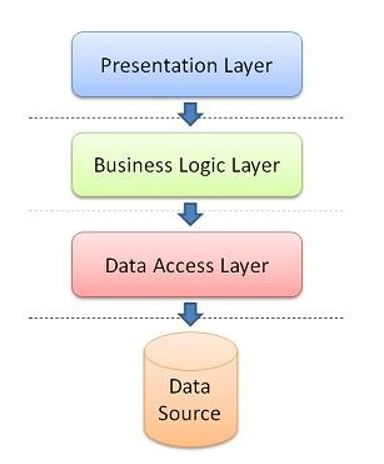
\includegraphics[scale=1]{immagini/layered_architecture}
	\caption{Schema architettura Layered 3-tier}
\end{figure}
L'architettura \textit{Layered 3-tier} è una architettura software molto semplice in cui le varie funzionalità sono separate logicamente ovvero suddivise su livelli logici differenti in comunicazione tra di loro.\\
I componenti all'interno di un'architettura di questo tipo sono organizzati in livelli orizzontali, ognuno dei quali si occupa di uno specifico ruolo all'interno del sistema completo.\\
Il pattern di questa tipologia di architettura non specifica il numero di livelli ma, nella versione più comune, il numero di livelli è tre suddiviso in: \textit{Presentation Layer}, \textit{Business Logic Layer} e \textit{Data Access Layer} il quale, poi, si occuperà di accedere ai dati all'interno del \textit{Data Source}.\\
Ogni livello, come abbiamo già visto, si occupa di uno specifico ruolo all'interno del sistema completo:
\begin{itemize}
	\item \textbf{Presentation Layer} - ha lo scopo di gestire l'interazione del sistema con il mondo esterno, in particolare con gli utenti. Include le maschere per visualizzare e inserire dati, controlli, dai più semplici ai più complessi, e i meccanismi per intercettare e gestire opportunamente tutti gli eventi che sono scatenati dalle azioni degli utenti;
	\item \textbf{Business Logic Layer} - include l'insieme delle regole di business che regolano il funzionamento dell'applicazione, intercetta le richieste provenienti dallo strato di presentazione e le gestisce opportunamente;
	\item \textbf{Data Access Layer} - conosce le modalità per leggere e salvare le informazioni interne al sistema nell'ambito di una sorgente dati (non necessariamente un database centralizzato).
\end{itemize}
\subsection{Analisi e rating dell'architettura scelta}
La seguente tabella contiene una valutazione delle principali caratteristiche dell'architettura scelta.\\
Andremo ora a spiegarle e ad analizzarle.
\begin{figure}[h]
	\centering
	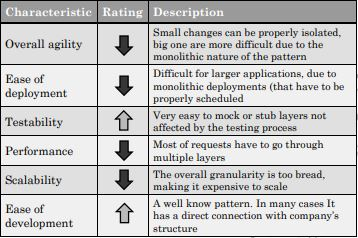
\includegraphics[scale=1]{immagini/layered_architecture_analysis}
	\caption{Analisi dell'architettura Layered 3-tier}
\end{figure}
\begin{itemize}
	\item \textbf{Overall agility}:
	\begin{itemize}
		\item \textbf{Rating}: Basso;
		\item \textbf{Analisi}: è la capacità del sistema di reagire velocemente ad un ambiente in costante cambiamento. Nonostante le modifiche siano isolate attraverso i livelli è comunque difficile apportare dei cambiamenti a causa della sua struttura monolitica della maggior parte delle implementazioni che lo adottano e dello stretto accoppiamento che si ha tra i livelli\cite{3tierArch}\cite{3tierArch2}.
		\item \textbf{Valutazione}: nonostante la non semplice gestione dei cambiamenti questo non è un problema per lo sviluppo del modulo \gls{ITF} in quanto, essendo il sistema sviluppato interamente appoggiandosi ad \textit{Ethereum}, le modifiche sono difficili di per sé a causa dell'immutabilità garantita ai contratti una volta che questi sono rilasciati nella rete.\\
		Per andare a modificare un contratto, l'unico modo è riscriverlo con tutte le modifiche necessarie e sostituire gli indirizzi nei contratti che lo utilizzano.\\
		Potrebbe risultare un procedimento complesso ma così non è se si adottano strategie che prevedono questo scenario (metodi di \textit{setting} degli indirizzi bloccati ai soli proprietari dei contratti).\\
	\end{itemize}
	Per questa motivazione nonostante il rating basso di questa caratteristica, il sistema non ne viene influenzato in modo negativo.
	\item \textbf{Ease of deployment}:
	\begin{itemize}
		\item \textbf{Rating}: Basso;
		\item \textbf{Analisi}: un piccolo cambiamento ad una componente può richiedere la ri-implementazione dell'intera applicazione o di una grossa porzione di essa, facendo sì che sia necessaria la pianificazione e l'implementazione durante ore non lavorative\cite{3tierArch}\cite{3tierArch2}.
		\item \textbf{Valutazione}: come per l'\textit{Overall agility} questa caratteristica non è un problema per l'implementazione del modulo se viene pensato per essere esteso in quanto, come detto nel punto precedente, essendo tutto appoggiato sopra la rete \textit{Ethereum} l'implementazione di nuovi contratti o la loro modifica necessità la creazione del contratto e la sostituzione degli indirizzi all'interno dei contratti che lo utilizzano.
	\end{itemize}
	\item \textbf{Testability}:
	\begin{itemize}
		\item \textbf{Rating}: Alto;
		\item \textbf{Analisi}: siccome i componenti sono suddivisi in livelli separati è possibile creare dei mockup o degli \emph{\gls{stub}}\glsfirstoccur per i livelli che dipendono direttamente da quello che si sta sviluppando. Questo fa sì che la testabilità del sistema sia molto facile\cite{3tierArch}\cite{3tierArch2}.\\
		\item \textbf{Valutazione}: essendo, la maggior parte del modulo, appoggiato ad \textit{Ethereum} ed essendo i contratti immutabili, una volta rilasciati nella rete, si ha la necessità di operare un gran numero di test prima del rilascio in modo da evitare di dover creare un nuovo contratto che va a sostituire quello contenente errori.\\
		Per questo motivo questa caratteristica è di fondamentale importanza per il modulo \gls{ITF}.		
	\end{itemize}
	Questa caratteristica è fondamentale per l'\gls{ITF} \textit{Ethereum} e il suo rating alto è stato uno dei motivi di scelta dell'intera architettura.
	\item \textbf{Performance}:
	\begin{itemize}
		\item \textbf{Rating}: Basso
		\item \textbf{Analisi}: il pattern architetturale non si presta bene nell'avere alte performance questo è dato dal fatto che ogni volta che si vuole interagire con un livello bisogna necessariamente passare attraverso multipli livelli per andare a soddisfare la richiesta\cite{3tierArch}\cite{3tierArch2}.
		\item \textbf{Valutazione}: il fatto di dover passare attraverso molti livelli senza dare la possibilità di "scavalcarne" alcuni per determinate richieste è un concetto chiave dell'architettura detto T\textit{he layers of Isolation}. Questo fa sì che ogni cambiamento ad un livello non abbia effetto su altri componenti di altri livelli: il cambiamento è isolato ai componenti interni al livello.\\
		Se si permettesse ad alcuni componenti di "scavalcare" i livelli direttamente sottostanti, i cambiamenti a questo livello influenzerebbero pesantemente tutti gli altri andando a creare un forte accoppiamento tra le parti.\\
		La considerazione da fare è che, il sistema che vogliamo realizzare, è semplice e non prevede una profondità dei livelli così alta da andare a inficiare pesantemente sulle prestazioni del modulo in più c'è da dire che la \textit{Blockchain Ethereum} è il vero freno sulle prestazioni del sistema in quanto, una transazione, potrebbe richiedere anche svariati minuti.
	\end{itemize}
	\item \textbf{Scalability}:
	\begin{itemize}
		\item \textbf{Rating}: Basso
		\item \textbf{Analisi}: la Scalabilità (capacità di un sistema di reagire a richieste di lavoro più pesanti) è un problema per i sistemi sviluppati tramite l'utilizzo di questa architettura. In un'architettura di questo tipo la scalabilità può essere ottenuta andando a dividere i vari livelli in implementazioni fisicamente separate o andando a replicare l'interna applicazione in nodi multipli\cite{3tierArch}\cite{3tierArch2}.
		\item \textbf{Valutazione}: questa caratteristica potrebbe essere l'unica in grado di andare ad intaccare il modulo \gls{ITF} se non pensato correttamente.\\
		Secondo me, il problema principale all'interno della rete \textit{Ethereum} alla quale ci andiamo ad appoggiare, è principalmente dovuto alla scrittura dei dati e quindi durante la fase di registrazione di un nuovo utente o l'aggiornamento dei certificati conseguiti.\\
		Queste essendo operazioni che avvengono con bassa frequenza (un utente si registra una sola volta in quanto l'identità digitale è unica ma condivisa per ogni servizio e l'inserimento di nuove certificazioni non è un'operazione che viene fatta di frequente) potrebbero non avere effetti negativi nel sistema in quanto, quello che viene fatto principalmente, sono letture di dati da parte dei vari Service Providers prima di permettere il rilascio di un servizio.
	\end{itemize}
	\item \textbf{Ease of development}:
	\begin{itemize}
		\item \textbf{Rating}: Alto
		\item \textbf{Analisi}: l'Ease of development (facilità di sviluppo) raggiunge livelli molto alti soprattutto data dal fatto che è un'architettura molto semplice e conosciuta.\\
		Siccome molte compagnie ed aziende sviluppano applicazioni e sistemi andando a separare i livelli per competenze, questo pattern diventa una delle scelte migliori\cite{3tierArch}\cite{3tierArch2}.
		\item \textbf{Valutazione}: la facilità di sviluppo di un sistema basato su questa architettura è, sicuramente, una caratteristica importante.\\
		Questo viene dal fatto che, grazie ad un'architettura del genere, è possibile andare a mettere le mani nel codice in tempi molto più brevi rispetto a quelli richiesti se venisse adotta un'altra tipologia di architettura.\\
		In più, il fatto di poter dividere i vari livelli per competenze permette lo sviluppo separato e parallelo di componenti diverse senza la necessità che il sistema segua un filo logico inizio – fine.\\
		Quest'ultimo accorgimento è di fondamentale importanza in quanto è stato necessario suddividere la parte fornt-end dal back-end e lo sviluppo è avvenuto in parallelo.
	\end{itemize}
\end{itemize}
\section{Approccio alla progettazione}
Per la progettazione del modulo si è deciso di utilizzare un approccio \emph{\gls{topDown}}\glsfirstoccur. Essa consiste nel descrivere il sistema partendo da una visione generale ad alto livello per poi scendere nel particolare delle parti individuate.\\
Nella visione ad alto livello è possibile notare che il sistema è composto da diversi packages che interagiscono tra di loro. Entrando nel dettaglio si vanno ad individuare tutte le componenti più piccole e semplici tramite la strategia \textit{divide-et-impera}. L'approccio \gls{topDown} parte dall'obiettivo e da esso valorizza il "perché" e fa dipendere il "come", permettendo di suddividere il lavoro rendendolo più comprensibile e, quindi, di più facile manutenibilità.
\section{Architettura generale}
Il modulo \gls{ITF} è formato da due parti distinte:
\begin{itemize}
	\item \textbf{Front-end}:l'applicativo tramite la quale gli utenti e gli attori esterni possono interagire con l'intero sistema;
	\item \textbf{Back-end}: tutte le componenti che contengono la \textit{Business Logic}, gestiscono la persistenza dei dati interni alla \textit{Blockchain Ethereum} e le componenti necessarie a far sì che il \textit{front-end} riesca ad interagire con la \textit{Business Logic}.
\end{itemize}
Il lato \textit{back-end} prevede l'utilizzo della \textit{Blockchain Ethereum} per la gestione e la certificazione delle informazioni personali dell'utente insieme alla verifica delle informazioni da parte di un Service Provider che ha ricevuto una richiesta di accesso da parte di un utente.\\
Tutte queste operazioni vengono gestite tramite \textit{smart contracts Solidity} in modo da permettere l'interazione con l'\gls{evm}.\\
Tutte le componenti della parte \textit{back-end} sono raggruppate in packages. Questo viene fatto perché, all'interno di ogni package, troviamo:
\begin{itemize}
	\item Gli \textit{smart contracts} che contengono i dati da gestire e dei metodi fittizi che contengono gli indirizzi ai metodi veri e propri;
	\item Gli \textit{smart contracts} contenenti l'implementazione vera e propria dei vari metodi.
\end{itemize}
Questo è necessario in quanto un contratto \textit{Ethereum}, una volta rilasciato nella rete, diventa immutabile e quindi non più modificabile in caso di malfunzionamenti o risultati inaspettati.\\
Separando la parte logica (metodi) dalla componente dati (con metodi fittizi) e collegando le due parti tramite indirizzi fa sì che l'eventuale presenza di errori possa essere gestita andando a implementare nuovamente solo la parte logica e cambiando gli indirizzi nella componente dati (questo cambiamento deve essere gestito tramite appositi metodi \textit{setter}).
\newpage
\section{Componenti del modulo}
\subsection{Visione generale}
\begin{figure}[!h]
	\centering
	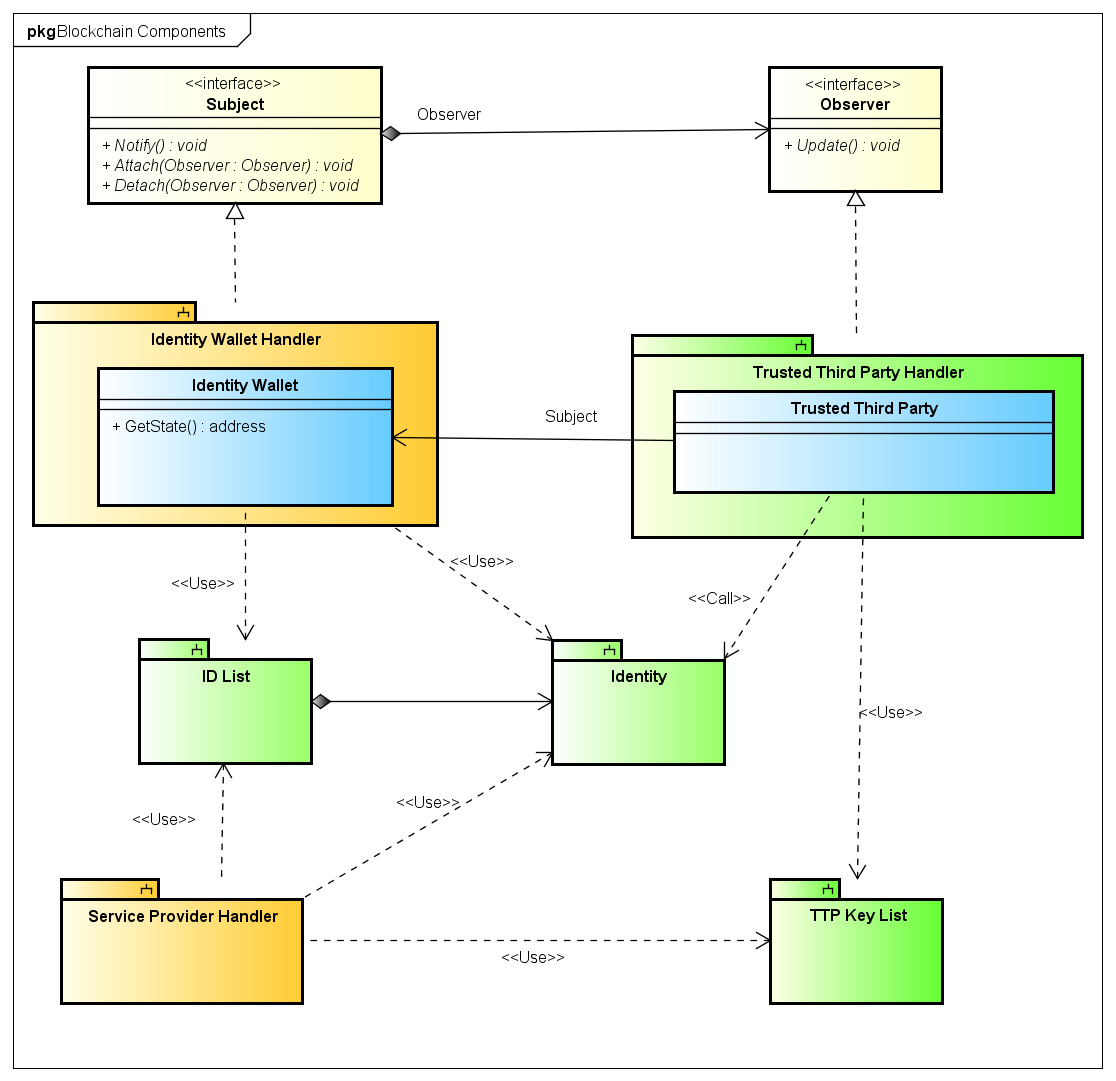
\includegraphics[scale=0.5]{immagini/architettura_alto_livello}
	\caption{Visione ad alto livello}
	\label{fig:visioneAltoLivello}
\end{figure}
\begin{itemize}
	\item \textbf{Descrizione}:\\
	Questo è il package principale dell'applicazione lato \textit{back-end}.\\
	Tutte le classi e i sottosistemi presenti in questo package contengono la \textit{business logic} e la persistenza dei dati necessari per realizzare il modulo \gls{ITF} e la sua interazione con il mondo esterno verso il Service Provider e l'Identity Wallet.
	\item \textbf{Package contenuti}:\\
	\begin{itemize}
		\item Identity Wallet Handler;
		\item Trusted Third Party;
		\item ID List;
		\item TTP Key List;
		\item Identity;
		\item Service Provider Handler.
	\end{itemize}	
\end{itemize}
Come si può vedere dallo schema in figura \ref{fig:visioneAltoLivello} le varie componenti presentano dei colori diversi. Questo è stato fatto per rendere più chiara la suddivisione dei package in base al \textit{design pattern} ad essi associati.\\
\begin{itemize}
	\item \textbf{Design pattern Observer} - formano questo design pattern: il package Identity Wallet Handler, la classe Trusted Third Party e le interfacce Subject e Observer (colore: azzurro);
	\item \textbf{Design pattern Façade} - formano questo design pattern i due package Service Provider Handler e Identity Wallet Handler (colore: arancione);
	\item \textbf{Desing pattern Strategy} - tutti i package nello schema presentano questo design pattern al loro interno quindi: Identity Wallet Handler, Service Provider Handler, ID List e Identity (colore verde).
\end{itemize}
Alcuni package non rispettano i colori sopracitati in quanto realizzano più di un design pattern. Vedremo in seguito quali.
\subsection{Identity Wallet Handler}
\begin{figure}[!h]
	\centering
	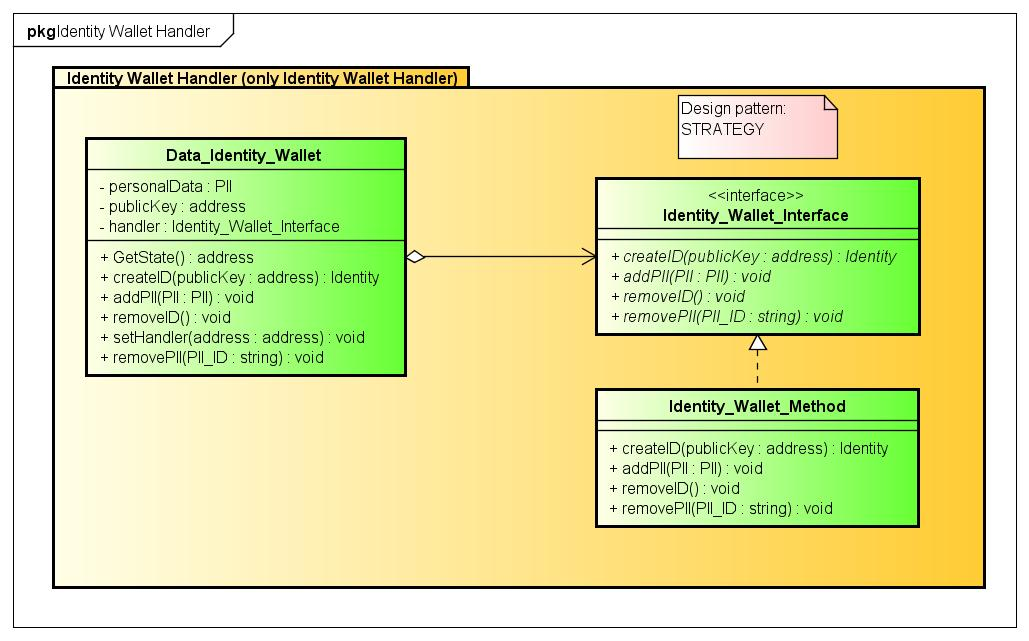
\includegraphics[width=0.8\textwidth]{immagini/identityWalletHandler}
	\caption{Schema Identity Wallet}
\end{figure}
\begin{itemize}
	\item \textbf{Descrizione}
	Package che modella l'interazione tra l'Identity Wallet ed il sistema esterno. Si occupa principalmente di tutte le attività che l'utente può fare all'interno della \textit{Blockchain Ethereum}.\\
	Contiene, al suo interno, tutte le classi necessarie affinché si riesca a mantenere separati le informazioni dai metodi.\\
	Il nome del package tra parentesi (only Identity Wallet Handler) è un modo per indicare la possibilità, che da \textit{Solidity}, di far eseguire le operazioni contenute in Data\_Identity\_Wallet solo dal Wallet stesso e non da altri contratti esterni.
	\item \textbf{Interazione con altre componenti}
	\begin{itemize}
		\item Trusted Third Party;
		\item ID List;
		\item Identity.
	\end{itemize}
	\item \textbf{Design pattern presenti}
	\begin{itemize}
		\item Façade (arancione);
		\item Strategy (verde);
		\item Singleton (non segnato);
		\item Observer (non segnato).
	\end{itemize}
\end{itemize}
\subsubsection{Data\_Identity\_Wallet}
\begin{itemize}
	\item \textbf{Descrizione}
	Componente che racchiude tutta l'essenza del package Identity Wallet Handler.
	Questa classe contiene metodi, informazioni riguardanti l'identità dell'utente e informazioni necessarie per l'interazione con il sistema.\\
	Per realizzare il modulo in \textit{Ethereum} è consigliato separare la \textit{business logic} e la persistenza dei dati. Questa componente mantiene principalmente tutti i dati necessari e delega, tramite \textit{strategy} pattern, la realizzazione dei metodi ad altre componenti.\\
	Il codice, se presenta dei bug o comportamenti anomali, non è possibile correggerlo. L'unico modo per risolvere è andare a rimpiazzare il vecchio contratto con uno nuovo e cambiare gli indirizzi dei client che utilizzavano il modulo precedente.\\
	Se la classe contenesse sia dati che metodi allora bisognerebbe rimpiazzare tutto il blocco perdendo così i dati degli utenti registrati.\\
	Separando la componente logica dai dati e collegando il tutto tramite pattern \textit{strategy} è possibile, in caso di errore, creare un nuovo Identity\_Wallet\_Method e, senza alcuna perdita di dati utente, ripristinare il normale funzionamento del modulo.	
	\item \textbf{Interazione con altre componenti}
	\begin{itemize}
		\item\textbf{ Identity\_Wallet\_Interface}: Questo contratto contiene la firma dei metodi che, le classi concrete che realizzano l'interfaccia, devono implementare per andare a soddisfare le richieste che vengono fatte dall'Identity Wallet tramite Data\_Identity\_Wallet.
		\item\textbf{ Identity\_Wallet\_Method}:Contratto che realizza le specifiche dell'interfaccia Identity\_Wallet\_Interface tramite l'implementazione concreta di tutti i metodi dichiarati.
	\end{itemize}
	\item \textbf{Design pattern presenti}\\
	Partecipa alla realizzazione del pattern \textit{strategy} interno al package Identity Wallet Handler e realizza, insieme alla classe Trusted Third Party, il design pattern \textit{Observer} necessario per la certificazione delle informazioni personali.
\end{itemize}
\subsection{ID List}
\begin{figure}[!h]
	\centering
	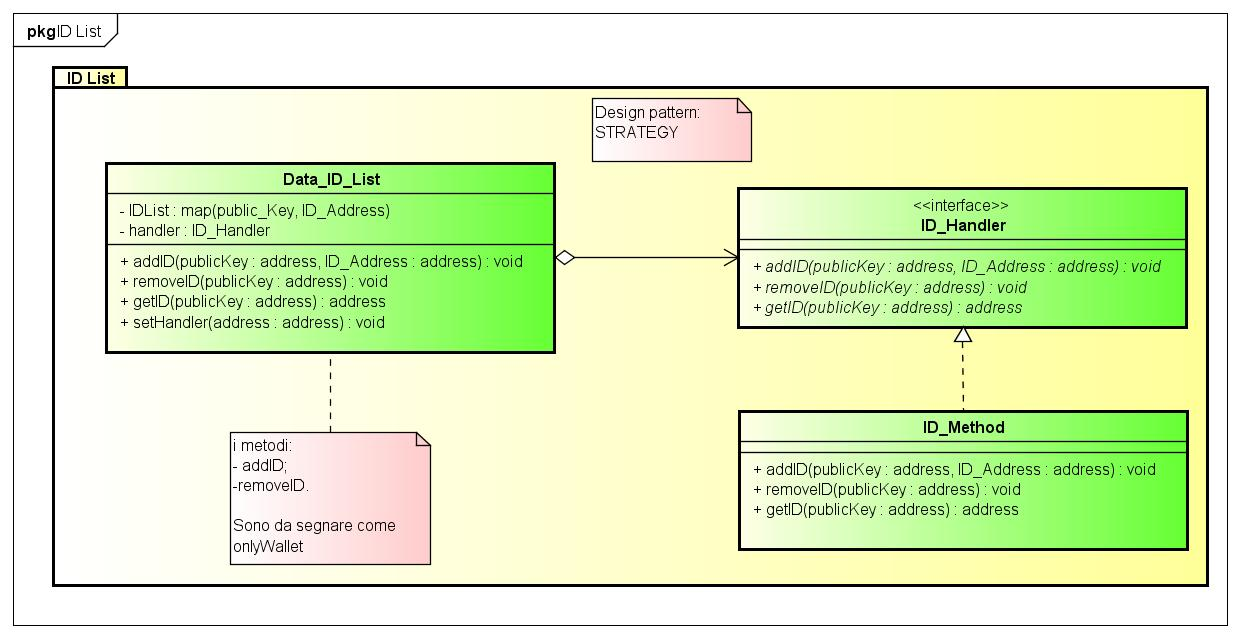
\includegraphics[width=0.8\textwidth]{immagini/idList}
	\caption{Schema ID List}
\end{figure}
\begin{itemize}
	\item \textbf{Descrizione}
	Package che fa da ponte tra le varie componenti interne al sistema. 
	Al suo interno contiene tutte le informazioni e i metodi necessari per far comunicare tra di loro l'Identity Wallet Handler, Trusted Third Party e Service Provider Handler.\\
	Come gli altri package, anche questo presenta il consueto \textit{strategy} pattern per separare la business logic e la persistenza dei dati.\\
	Un altro design pattern che questa componente realizza è il \textit{singleton} in quanto è utilizzata da tutte le altre componenti per recuperare le informazioni delle identità utente che essa contiene.\\
	Alcuni metodi di questo package sono segnati come onlyWallet ovvero con il permesso reso disponibile da \textit{Solidity} che fa sì che sia possibile specificare quale componente può invocare i metodi, rigettando le chiamate da tutti gli altri contratti non specificati.
	\item \textbf{Interazione con altre componenti}
	\begin{itemize}
		\item Identity Wallet Handler;
		\item Identity;
		\item Trusted Third Party;
		\item Service Provider Handler.
	\end{itemize}
	\item \textbf{Design pattern presenti}\\
	Partecipa alla realizzazione del design pattern \textit{strategy} ed è un \textit{singleton} per recuperare tutte le informazioni riguardanti le identità digitali degli utenti.
\end{itemize}
\subsubsection{Data\_ID\_List}
\begin{itemize}
	\item \textbf{Descrizione}
	Rappresenta la componente principale di tutto il package ID List in quanto si occupa sia della gestione dei dati che dell'invocazione dei metodi.\\
	Questa componente si occupa principalmente di mantenere una mappatura tra l'identità dell'utente (rappresentata da un indirizzo \textit{Ethereum}) e la corrispondente identità nell'Identity Wallet (rappresentata da una chiave pubblica). Queste informazioni vengono conservate all'interno di una mappa che associa i due tipi di informazioni per ogni utente registrato al sistema.\\
	Oltre a questo, troviamo anche i metodi necessari per poter inserire, rimuovere e recuperare l'identità utente.\\
	Partecipando ad un design pattern \textit{strategy} i metodi interni a questa componente delegano l'esecuzione a ID\_Method in modo da preservare la separazione tra dati e business logic.
	\item \textbf{Interazione con altre componenti}
	\begin{itemize}
		\item \textbf{ID\_Handler}: Interfaccia necessaria per la realizzazione del pattern \textit{strategy} interno al package ID List.\\
		Contiene le firme di tutti i metodi che sono utilizzati da Data\_ID\_List e che sono realizzati, concretamente, dalla componente ID\_Method.
		\item \textbf{ID\_Method}: Classe che implementa i metodi necessari per recuperare, inserire ed eliminare le informazioni associate alle identità utente.\\
		Realizza, concretamente, tutti i metodi richiamati dal Data\_ID\_List ed esposti dall'interfaccia ID\_Handler.
	\end{itemize}
	\item \textbf{Design pattern presenti}\\
	Realizza il design pattern \textit{strategy} interno al package.
\end{itemize}
\subsection{Identity}
\begin{figure}[!h]
	\centering
	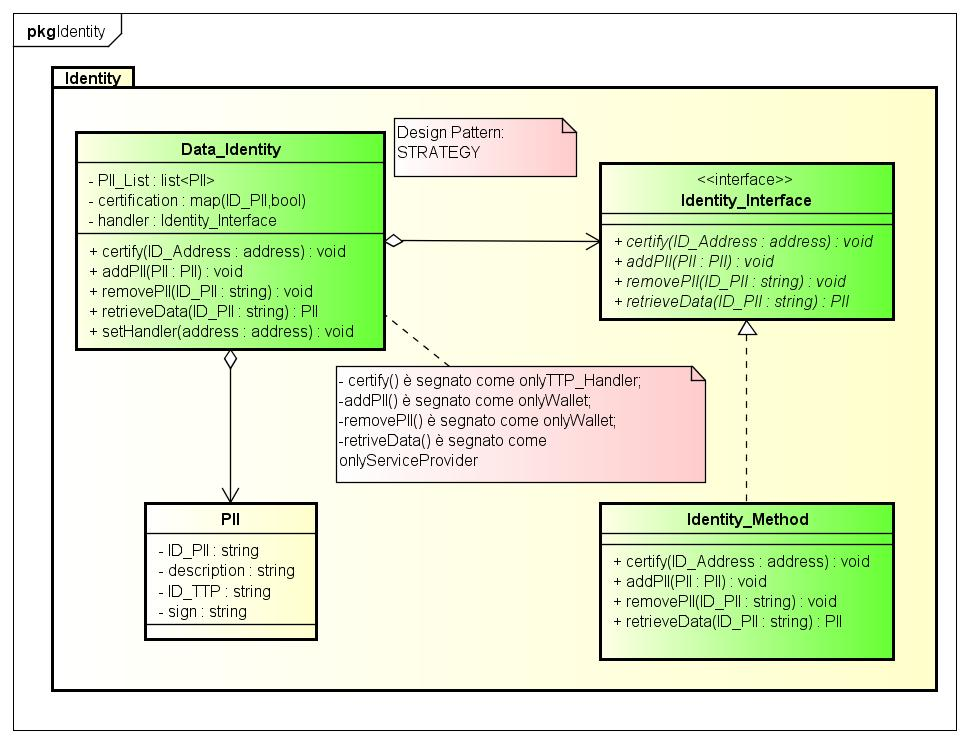
\includegraphics[width=0.8\textwidth]{immagini/identity}
	\caption{Schema Identity}
\end{figure}
\begin{itemize}
	\item \textbf{Descrizione}
	Package che contiene tutti i dati e le informazioni personali relative all'identità di un utente e tutti i metodi necessari, agli altri package, per poter aggiungere, rimuovere, certificare e verificare le \gls{PII}.\\
	Questo è un altro dei package core del sistema \gls{ITF} che si vuole realizzare in quanto, insieme all'Identity\_Wallet\_Handler crea e gestisce le identità degli utenti.\\
	Anche in questo package possiamo trovare il solito design pattern \textit{strategy} per poter mantenere separati la \textit{business logic} dai dati modellati dal package.
	\item \textbf{Interazione con altre componenti}
	\begin{itemize}
		\item Identity Wallet Handler;
		\item Trusted Third Party Handler;
		\item ID List;
		\item Service Provider Handler.
	\end{itemize}
	\item \textbf{Design pattern presenti}\\
	Al suo interno troviamo il design pattern \textit{strategy} per mantenere separati \textit{business logic} e persistenza dei dati.
\end{itemize}
\subsubsection{Data\_Identity}
\begin{itemize}
	\item \textbf{Descrizione}
	Classe che modella tutto il package Identity in quanto contiene sia i dati riguardanti un utente (le sue \gls{PII} sotto forma di lista) sia tutti i metodi necessari per la realizzazione della business logic del modulo \gls{ITF} (con delega ad oggetti concreti di tipo Identity\_Method).\\
	Come per gli altri package, anche questa componente partecipa alla realizzazione di un design pattern \textit{strategy} necessario per mantenere separate le due componenti sopracitate in modo da poter correggere eventuali errori o malfunzionamenti e per permettere, in futuro, l'espansione delle funzionalità del package.
	\item \textbf{Interazione con altre componenti}
	\begin{itemize}
		\item \gls{PII}: Rappresenta un'informazione personale che appartiene ad un determinato utente.\\
		Le informazioni personali che vengono rappresentate vanno dal semplice nome e cognome fino a certificazioni o attestati conseguiti dall'utente che si sta esaminando.\\
		Queste informazioni formano, all'interno di Data\_Identity, una lista di \gls{PII} che rappresentano il profilo identificativo di un utente che vuole accedere ad un determinato servizio.		
		\item \textbf{Identity\_Interface}: Interfaccia che espone tutti i metodi necessari a Data\_Identity per poter realizzare la \textit{business logic} del package Identity tramite delega ad un oggetto che realizza concretamente l'interfaccia (Identity\_Method).
		\item \textbf{Identity\_Method}: Classe che realizza concretamente i metodi esposti dall'interfaccia Identity\_Interface e che sono necessari a Data\_Identity per andare a realizzare la business logic del modulo.\\
		Questa componente realizza il design pattern \textit{strategy} interno al modulo.\\
		I metodi implementati dovranno essere segnati con particolari privilegi in modo che non tutti i contratti (interni o esterni al sistema \gls{ITF}) possano invocarli e gestire i dati personali degli utenti.	
	\end{itemize}
	\item \textbf{Design pattern presenti}\\
	Partecipa alla realizzazione del design pattern \textit{strategy}.
\end{itemize}
\subsection{TTP Key List}
\begin{figure}[!h]
	\centering
	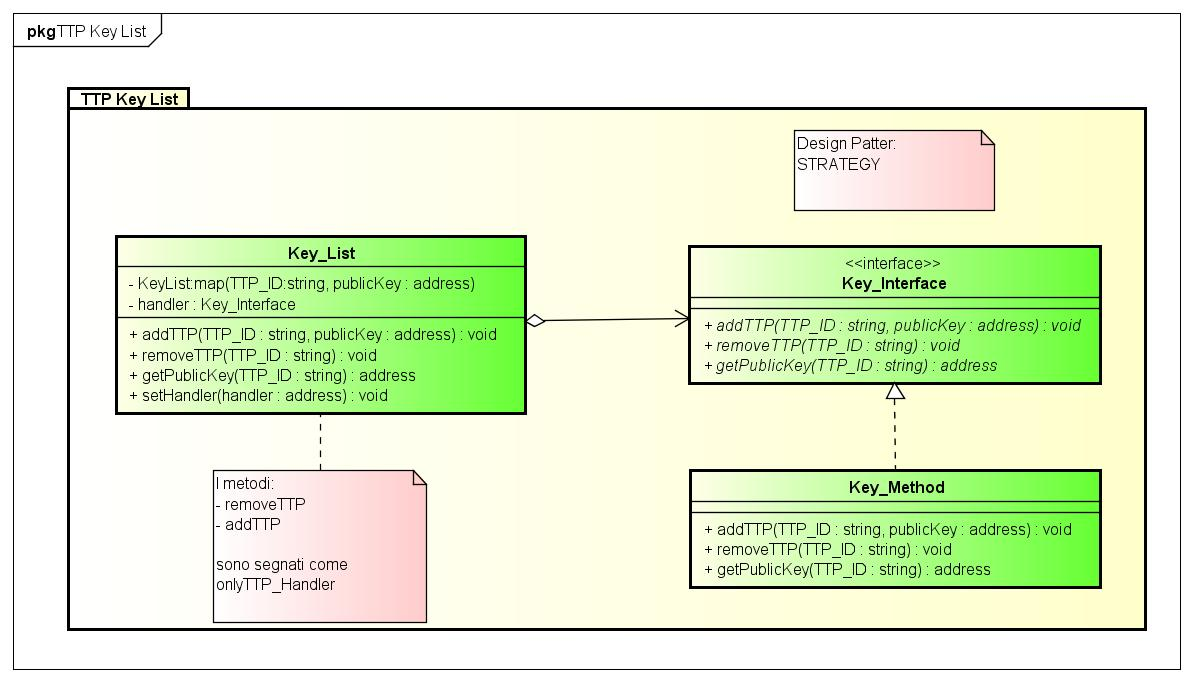
\includegraphics[width=0.8\textwidth]{immagini/ttpkeylist}
	\caption{Schema TTP Key List}
\end{figure}
\begin{itemize}
	\item \textbf{Descrizione}
	Questa componente fa da tramite tra il Service Provider Handler e Trusted Third Party Handler.
	Ogni qual volta un Service Provider desidera recuperare le informazioni di un utente e vuole verificare che, contenute nel suo oggetto Identity, siano certificate recupera, tramite TTP Key List, la chiave pubblica dell'ente certificatore che ha certificato le informazioni dell'utente e, tramite un confronto con la firma posta nelle informazioni personali dell'utente (firma = hash(dati utente + chiave privata \gls{TTP})), controlla che le informazioni siano effettivamente state firmate dall'ente che è stato segnato come certificatore per quelle informazioni.\\
	Quindi, questa componente, è di fondamentale importanza per permettere il sistema di verifica e certificazione che il modulo \gls{ITF} deve implementare.\\
	Anche questa componente, come tutte le altre, viene implementata tramite uno \textit{strategy} pattern in modo da mantenere separata la logica e i dati che rappresentano l'associazione \gls{TTP} - chiave pubblica.\\
	Oltre a questo
	\item \textbf{Interazione con altre componenti}
	\begin{itemize}
		\item Service Provider Handler;
		\item Trusted Third Party Handler.
	\end{itemize}
	\item \textbf{Design pattern presenti}\\
	All'interno del package TTP Key List troviamo il design pattern \textit{strategy} ed è un \textit{singleton} per recuperare tutte le informazioni riguardanti gli enti certificatori autorizzati.
\end{itemize}
\subsubsection{Key\_List}
\begin{itemize}
	\item \textbf{Descrizione}
	Componente che gestisce tutto il package TTP Key List in quanto contiene sia i dati che i metodi necessari per recuperare tutte le informazioni necessarie per andare a verificare le informazioni personali dell'utente.\\
	La parte principale di questa componente sono principalmente i dati che rappresentano l'associazione tra l'identificativo univoco di un ente certificatore e la sua chiave pubblica necessaria per andare a verificare i dati.\\
	Insieme a questo contiene tutti i metodi, segnati come onlyTTP\_Handler, che servono per andare ad inserire, rimuovere e recuperare tutte le informazioni riguardo una Trusted Third Party.\\
	Come le altre componenti, anche questa delega l'implementazione dei metodi ad una componente terza il Key\_Method.
	\item \textbf{Interazione con altre componenti}
	\begin{itemize}
		\item \textbf{Key\_Interface}: Interfaccia che espone tutti i metodi necessari a Key\_List per poter recuperare, inserire e rimuovere le informazioni relative alle Trusted Third Party che certificano le informazioni personali degli utenti.\\
		È una delle componenti necessarie per andare a realizzare il design pattern I del package TTP Key List che separa dati da business logic.
		\item \textbf{Key\_Method} :Classe che realizza i metodi esposti dall'interfaccia Key\_Interface e che sono richiamati dalla classe Key\_List per implementare la business logic del package TTP Key List.
	\end{itemize}
	\item \textbf{Design pattern presenti}\\
	Componente che partecipa alla realizzazione del design pattern \textit{strategy} ed è un \textit{singleton} per recuperare tutte le informazioni riguardanti gli enti certificatori autorizzati.
\end{itemize}
\subsection{Trusted Third Party Handler}
\begin{figure}[!h]
	\centering
	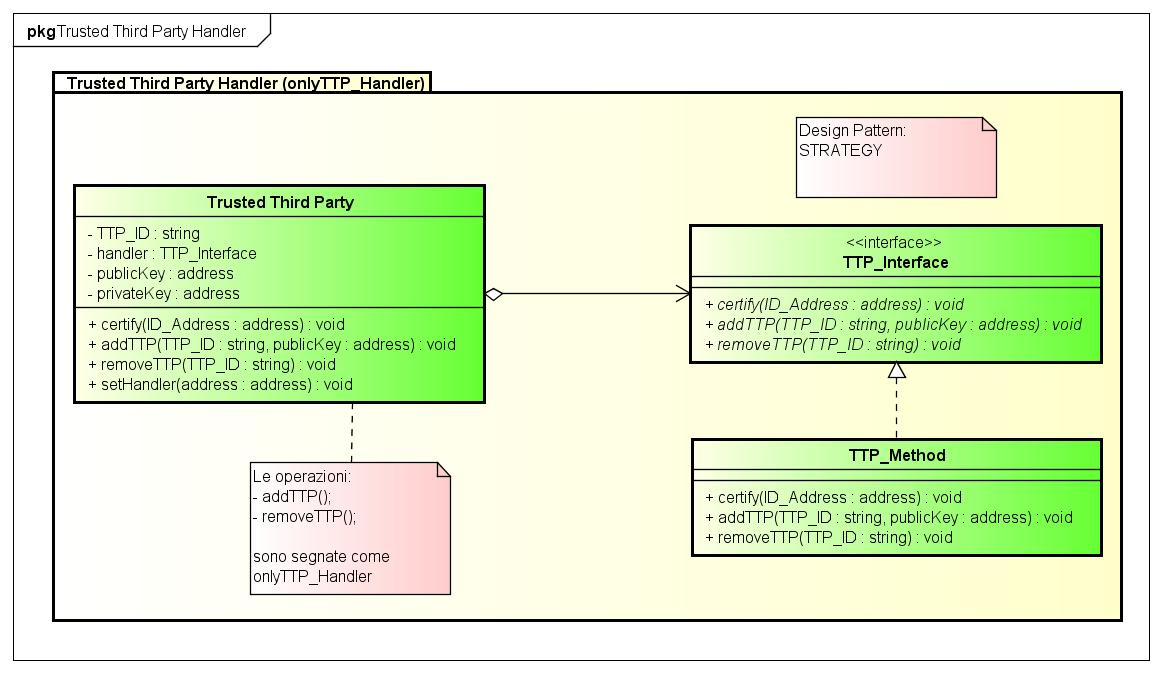
\includegraphics[width=0.8\textwidth]{immagini/trustedThirdPartyScheme}
	\caption{Schema Trusted Third Party}
\end{figure}
\begin{itemize}
	\item \textbf{Descrizione}
	Questa componente è necessaria per realizzare il pattern \textit{Observer} necessario per il funzionamento dell'intero sistema.\\
	La \gls{TTP} viene inserita all'interno di questo pattern in quanto, ogni qual volta un utente inserisce una nuova certificazione o un'informazione personale, in automatico viene notificata la Trusted Third Party.\\
	Questa, grazie all'indirizzo che gli viene passato dall'Identity Wallet Handler, recupera tutte le informazioni riguardanti l'identità di quell'utente e certifica le informazioni personali, appena aggiunte, ponendo la propria firma.\\
	Alcuni metodi di questo package come l'aggiunta e la rimozione di un ente certificatore dal sistema, sono segnati come onlyTTP\_Handler grazie alla funzionalità di proprietà di \textit{Solidity} che impedisce l'invocazione di metodi all'infuori del proprietario del contratto.
	\item \textbf{Interazione con altre componenti}
	\begin{itemize}
		\item Identity Wallet Handler;
		\item TTP Key List;
		\item Identity.
	\end{itemize}
	\item \textbf{Design pattern presenti}\\
	Seconda componente necessaria per la ralizzazione del pattern \textit{Observer}.
\end{itemize}
\subsubsection{Trusted Third Party}
\begin{itemize}
	\item \textbf{Descrizione}
	Componente interna al package Trusted Third Party Handler che ha lo scopo di mantenere al suo interno tutte le informazioni necessarie per poter certificare tutte le informazioni e certificazioni personali dell'utente.\\
	Contiene sia dati che invocazioni a metodi.\\
	I dati qui contenuti rappresentano, in modo univoco, l'ente certificatore (ID e Public Key) e il modo tramite la quale riesce a certificare i dati utente (Private Key).\\
	Per mantenere separata la \textit{business logic} dai dati partecipa come componente ad uno strategy pattern.
	\item \textbf{Interazione con altre componenti}
	\begin{itemize}
		\item \textbf{TTP\_Interface}: Interfaccia che contiene la firma dei metodi che il pattern \textit{strategy} deve realizzare all'interno del package Trusted Third Party Handler.\\
		Contiene tutti i metodi realizzati da TTP\_Method e richiamati da Trusted Third Party.		
		\item \textbf{TTP\_Method}: Componente concreta che realizza i metodi esposti dall'interfaccia TTP\_Interface e richiamati dal componente Trusted Third Party.\\
		Questa componente è fondamentale per andare a realizzare il design pattern \textit{strategy} che troviamo all'interno del package Trusted Third Party Handler
	\end{itemize}
	\item \textbf{Design pattern presenti}\\
	Partecipa alla realizzazione del design pattern \textit{strategy} interno al package.
\end{itemize}
\newpage
\subsection{Service Provider Handler}
\begin{figure}[!h]
	\centering
	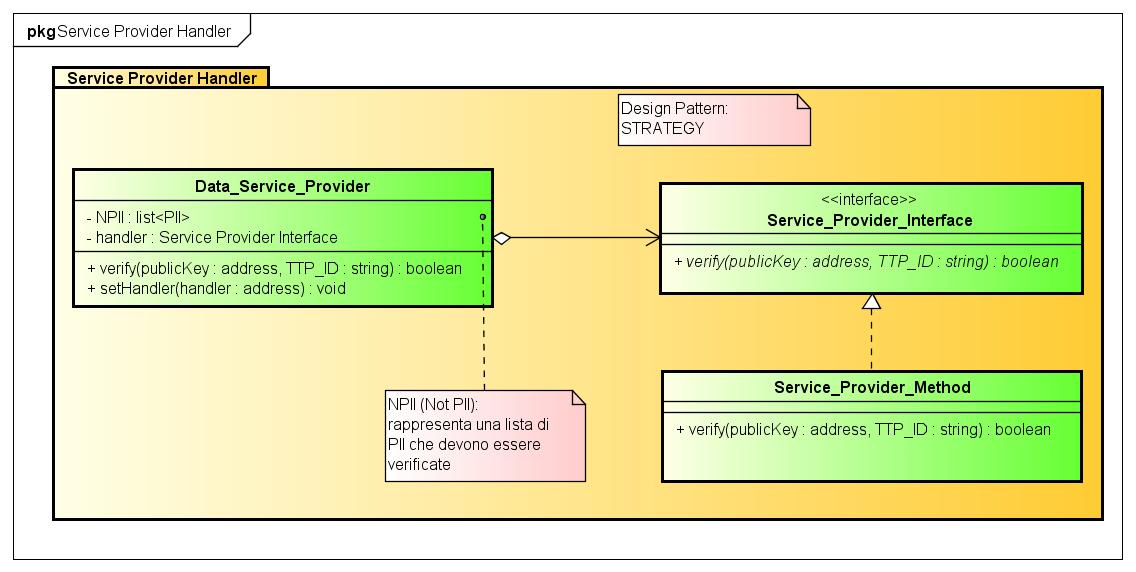
\includegraphics[width=0.8\textwidth]{immagini/serviceproviderhandler}
	\caption{Schema Service Provider}
\end{figure}
\begin{itemize}
	\item \textbf{Descrizione}
	Questo package è modella tutte le interazioni che avvengono tra il mondo esterno e la \textit{Blockchain Ethereum} che modella il sistema \gls{ITF}. In particolare modella tutte le operazioni che un Service Provider deve effettuare prima di erogare i suoi servizi ad un particolare utente.\\
	Per questo motivo, oltre che il consueto \textit{strategy} pattern questo package implementa anche il design pattern \textit{façade} per permettere l'interazione tra il presentation layer lato Serivce Provider e il sistema interno alla \textit{Blockchain Ethereum}.\\
	L'operazione principale che viene effettuata da questi componenti è la verifica delle informazioni personali di un utente (\gls{PII}) per accertarsi che siano certificate (firmate da un ente certificatore fidato).
	\item \textbf{Interazione con altre componenti}
	\begin{itemize}
		\item ID List;
		\item Identity;
		\item TTP Key List.
	\end{itemize}
	\item \textbf{Design pattern presenti}\\
	Oltre al consueto pattern \textit{strategy} questo contratto funge anche da \textit{façade} tra l'\gls{ITF} e il mondo esterno dalla parte di un Service Provider.
\end{itemize}
\subsubsection{Data\_Service\_Provider}
\begin{itemize}
	\item \textbf{Descrizione}
	Classe principale del package \textit{Service Provider Handler} che divide, grazie al pattern \textit{strategy},
	la\textit{ business logic} dai dati.\\
	La \textit{business logic} di questa classe rappresenta la funzionalità di verifica delle informazioni
	che un \textit{Service Provider} deve eseguire prima di erogare i suoi servizi ad un utente.\\
	I dati, invece, rappresentano la lista di \gls{PII} che un \textit{Service Provider} richiede essere certificati
	da parte di un ente certificatore fidato.\\
	La\textit{ business logic} viene implementata delegando la risoluzione del metodo ad un oggetto
	terzo in modo da prevenire errori o comportamenti anomali del codice.
	\item \textbf{Interazione con altre componenti}
	\begin{itemize}
		\item Service\_Provider\_Interface:Interfaccia che espone tutti i metodi necessari a Data\_Service\_Provider per poter implementare le funzionalità di verifica richieste dal Service Provider prima di erogare i servizi ad un utente.
		\item Service\_Provider\_Method:Classe concreta che implementa tutti i metodi esposti da Data\_Service\_Interface e che sono necessari a Data\_Service\_Provider per poter implementare la business logic del package Service Provider Handler.
	\end{itemize}
	\item \textbf{Design Pattern presenti}\\
	Componente necessaria per implementare il design pattern \textit{strategy}.
\end{itemize}
\section{Design Pattern}
In questa sezione vengono descritti i design pattern utilizzati per la realizzazione del prodotto. I design pattern sono delle soluzioni progettuali generali a problemi ricorrenti che possono essere adottati durante lo sviluppo del proprio sistema.
\subsection{Singleton}
\begin{itemize}
	\item \textbf{Scopo di utilizzo}: il pattern Singleton assicura che una certa classe abbia una sola istanza e fornisce ad essa un punto d’acceso globale.
	\item \textbf{Contesto}: all'interno dell'applicazione questo pattern viene usato per garantire la presenza di un unica istanza dei contratti TTP Key List e ID List.
\end{itemize}
\subsection{Façade}
\begin{itemize}
	\item \textbf{Scopo di utilizzo}: consente di definire un'interfaccia ad alto livello che semplifica l'accesso alle funzionalità erogate dal sottosistema e che fornisce un entry-point unico al sottosistema stesso;
	\item \textbf{Contesto}: per la realizzazione del modulo \gls{ITF} l'utilizzo di un design pattern di questo tipo è necessario in quanto bisogna far sì che l'utente riesca ad interagire con la \textit{Blockchain Ethereum} senza che si preoccupi della complessità del sistema e delle logiche che governano questo tipo di tecnologia come la gestione degli \emph{\gls{ether}}\glsfirstoccur, del \emph{\gls{gas}}\glsfirstoccur, spesa degli \gls{ether} per le transazioni.
\end{itemize}
\subsection{Strategy}
\begin{itemize}
	\item \textbf{Scopo di utilizzo}: Il pattern Strategy permette di definire una famiglia di algoritmi, di incapsularli e renderli intercambiabili fra loro. Questo pattern consente agli algoritmi di variare in modo indipendente rispetto al loro contesto di utilizzo, fornendo un basso accoppiamento tra le classi partecipanti.
	\item \textbf{Contesto}: la motivazione che ha portato alla scelta di questo pattern, è il fatto che, ogni qual volta qualcosa viene inserito all'interno della rete \textit{Blockchain Ethereum} diventa immutabile.\\
	Per questo motivo si è deciso di strutturare tutto il sistema in package che, al loro interno, dividessero i dati dall'implementazione dei metodi.\\
	Questo viene fatto perché se un metodo contiene errori o comportamenti anomali, sarebbe necessario sostituire tutto il contratto, perdendo anche tutti i dati utente fino ad ora accumulati.\\
	Tramite pattern Strategy e alle funzionalità di \textit{Solidity} è possibile separare queste due componenti e, tramite indirizzi, far sì che sia una componente terza a implementare concretamente i metodi.
	In caso di errori o comportamenti anomali è sufficiente creare un nuovo contratto da aggiungere alle componenti che ereditano dall'interfaccia che realizza lo Strategy e far sì che sia questa nuova componente ad eseguire i metodi che vengono chiamati	
\end{itemize}
\subsection{Observer}
\begin{itemize}
	\item \textbf{Scopo di utilizzo}: Il pattern Observer permette di definire una dipendenza uno a molti fra oggetti, in modo tale che se un oggetto cambia il suo stato interno, ciascuno degli oggetti dipendenti da esso viene notificato e aggiornato automaticamente.
	\item \textbf{Contesto}: All'interno del modulo \gls{ITF} questa tipologia di design pattern è richiesta nel momento in cui un utente si registra ed inserisce, o aggiorna, le sue \gls{PII}.\\
	In automatico, un oggetto \gls{TTP}, deve essere notificato del fatto che è avvenuta l'aggiunta di nuove informazioni così da poterle certificare per essere utilizzate da un Service Provider quando vuole erogare un servizio ad un utente che lo richiede.
\end{itemize}